\section{Magnesium chloride solutions in DME}
\label{section:mg-cl-dme-structural}

Magnesium salt solutions in organic liquids, such as dimethoxyethane (DME) were studied as possible electrolytes for novel batteries~\cite{roentgen-exp,mg-cl-dme-exp-1,mg-cl-dme-exp-2,mg-cl-dme-exp-3,mg-cl-dme-exp-4,mg-cl-dme-exp-5}. In particular, systems with Mg(TFSI)$_2$ with MgCl$_2$ addition were experimentally investigated~\cite{mg-dme-structures}. The data obtained shown that DME promotes aggreagates formation such as Mg$_2$Cl$_2^{2+}$ or Mg$_3$Cl$_4^{2+}$. The structures of such complexes are important because they differ in electrochemical activity. The results described here were part of the study done with QC and MD methods published in the article~\cite{mg-cl-dme}.

\subsection{System details}

QC calculations were performed with use of both the PBE and the B3LYP functionals for systems in vacuum, in the implicit solvent with $\varepsilon = 7.2$ modeled by the IEFPCM method~\cite{iefpcm} and for three systems containing explicit DME molecules with structures taken from crystallographic data in~\cite{mg-dme-structures}. The three latter structures were investigated in vacuum (explicit solvent) or embedded in the PCM solvent (hybrid solvent model).

\begin{table}[ht]
    \centering
    \caption{Compositions of Mg(TFSI)$_2$-MgCl$_2$-DME solutions}
    \label{tab:mg-cl-dme-compositions}
    \begin{tabular}{ccccc}
      \toprule
      \multicolumn{5}{c}{classical MD} \\
      system & Mg$^{2+}$ & TFSI$^{-}$ & Cl$^{-}$ & DME \\
      \midrule
      I & 61 & 82 & 40 & 500 \\
      II, IIa & 86 & 86 & 86 & 500 \\
      III, IIIa, IIIb, IIIc & 141 & 94 & 188 & 500 \\
      \midrule
      \multicolumn{5}{c}{ab initio MD} \\
      system & Mg$^{2+}$ & TFSI$^{-}$ & Cl$^{-}$ & DME \\
      \midrule
      III, IIIa, IIIb, IIIc & 3 & 2 & 4 & 30 \\
      \bottomrule
    \end{tabular}    
\end{table}

Classical MD simulations in DP-FF were performed at pressure 1~atm and temperature 298~K with a~time step of 0.5~fs for 400~ns for each system. Three types of systems with Mg salts dissolved in DME, varying in the Mg:Cl ratio, were constructed:
\begin{enumerate}[label=\MakeUppercase{\roman*}]
    \item --- mixture of 0.5~M Mg(TFSI)$_2$ and 0.25~M MgCl$_2$
    \item --- mixture of 0.5~M Mg(TFSI)$_2$ and 0.5~M MgCl$_2$
    \item --- mixture of 0.5~M Mg(TFSI)$_2$ and 1~M MgCl$_2$
\end{enumerate}
In the initial structures of these systems ions were randomly distributed. In addition, 4~other systems were simulated: IIa with Mg$^{2+}$ and Cl$^{-}$ initially in the form of Mg$_2$Cl$_2^{2+}$ complex, IIIa with initial mixture of MgCl$_2$ and Mg$_2$Cl$_2^{2+}$ complexes, IIIb with form (I) and IIIc with form (II) of the complex Mg$_3$Cl$_4^{2+}$ (these forms are described in the next subsection).

AIMD simulations were performed in the NVT ensemble for III, IIIa, IIIb and IIIc systems with smaller number of atoms than in classical MD. The size of the periodic simulation box was set to reproduce the densities of electrolytes obtained in classical MD simulations. Time step of 1~fs was used, and for each of the systems 35~ps of the simulation was recorded.

The compositions of the systems are listed in Table~\ref{tab:mg-cl-dme-compositions}. Presented RDFs were averaged over the last 20~ns or 30~ps for classical MD and AIMD respectively.

\subsection{Results}

\begin{figure}[H]
    \centering
    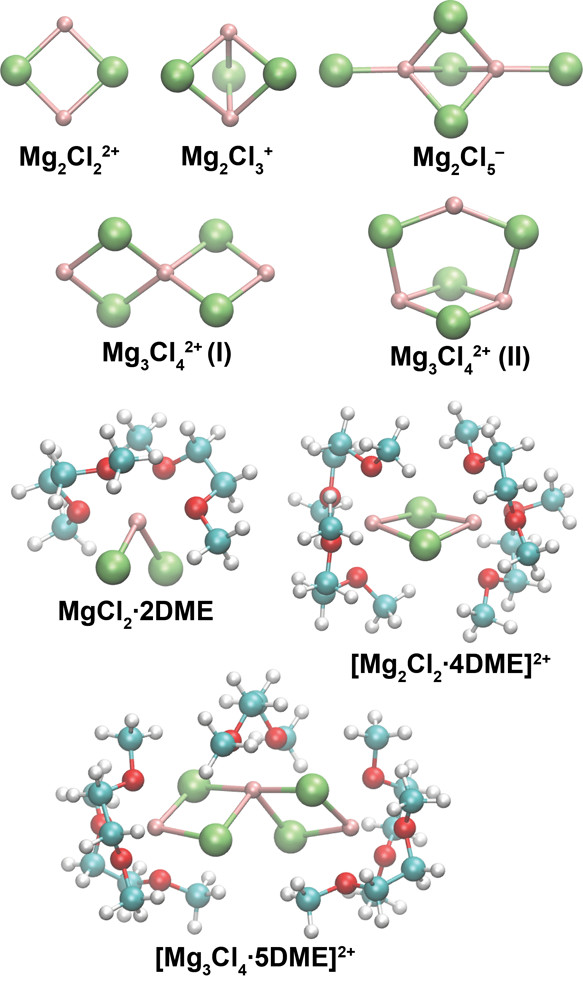
\includegraphics[width=0.4\textwidth]{img/3-structural-data-from-md-simulations/3-mg-cl-dme/complex-structures.png}
    \caption{Structures of Mg:Cl complexes studied by QC methods}
    \label{fig:mg-cl-dme-structures}
\end{figure}

Figure~\ref{fig:mg-cl-dme-structures} presents the structures of the complexes considered in QC calculations. For Mg$_3$Cl$_4^{2+}$ two stable geometries were found --- with Mg$^{2+}$ in linear order (form I) or triangular (form II). The results of geometry optimization in the PBE functional for selected structures are collected in Table~\ref{tab:mg-cl-dme-distances}. For the system with Mg$_3$Cl$_4^{2+}$ with DME molecules, only structure (I), found in the experiment, was considered. The distances between Mg$^{2+}$ ions are in the range 3.2-3.6~{\AA} and between Mg$^{2+}$ and Cl$^{-}$ in the range 2.2-2.5~{\AA}. These distances increase in solvent, for Mg-Mg by 0.2 and 0.3-0.35~{\AA} in PCM and explicit solvent, respectively, and for Mg-Cl by 0.1 and 0.15~{\AA}. For structures containing DME molecules, there are almost no changes between vacuum and PCM, what suggests, that the explicit solvent molecules are sufficient here to describe the solvent effect on interionic distances. Cl-Cl distances are less affected by the solvent, the effect is remarkable only for MgCl$_2$ where presence of explicit solvent molecules change the geometry from linear to bend. In systems with explicit DME molecules, distances between Mg$^{2+}$ ions and oxygen atoms from DME (O$_E$) decrease in PCM with respect to vacuum values.

\begin{table}
    \centering
    \caption[Interatomic distances (in \AA) for chosen complexes]{Interatomic distances (in \AA) for chosen complexes optimized with PBE functional}
    \label{tab:mg-cl-dme-distances}
\begin{tabular}{ccccc}
\toprule
\multicolumn{5}{c}{vacuum}                                                                                                                                                                                                                                                                                                                                                                                 \\
Structure   & Mg-Mg                                                           & Mg-Cl                                                                                                                          & Cl-Cl                                                                               & Mg-O$_{\text{E}}$                                                                                             \\
\midrule
MgCl$_2$       &                                                                 & 2 x 2.206                                                                                                                      & 4.412                                                                               &                                                                                                     \\
{[}MgCl$_2 \cdot$ 2E{]}    &                                                                 & 2.351, 2.367                                                                                                                   & 3.910                                                                               & \begin{tabular}[c]{@{}c@{}}2.208, 2.163\\ 2.337, 2.339\end{tabular}                                 \\
Mg$_2$Cl$_2^{2+}$      & 3.175                                                           & 4 x 2.358                                                                                                                      & 3.486                                                                               &                                                                                                     \\
{[}Mg$_2$Cl$_2 \cdot$ 4E{]}$^{2+}$   & 3.534                                                           & \begin{tabular}[c]{@{}c@{}}2.467, 2.468,\\ 2.476, 2.479\end{tabular}                                                           & 3.456                                                                               & \begin{tabular}[c]{@{}c@{}}2.140, 2.143,\\ 2 x 2.145,\\ 2.146, 2.147,\\ 2.153, 2.156\end{tabular}   \\
Mg$_3$Cl$_4^{2+}$ (I)  & \begin{tabular}[c]{@{}c@{}}2 x 3.208,\\ 6.415\end{tabular}      & \begin{tabular}[c]{@{}c@{}}4 x 2.298,\\ 4 x 2.452\end{tabular}                                                                 & \begin{tabular}[c]{@{}c@{}}2 x 3.500,\\ 4 x 4.234\end{tabular}                      &                                                                                                     \\
Mg$_3$Cl$_4^{2+}$ (II) & \begin{tabular}[c]{@{}c@{}}3.145,\\ 2 x 3.638\end{tabular}      & \begin{tabular}[c]{@{}c@{}}2 x 2.307,\\ 4 x 2.369,\\ 2 x 2.424,\\ 2 x 4.002,\\ 2 x 4.380\end{tabular}                          & \begin{tabular}[c]{@{}c@{}}3.486,\\ 4 x 3.836,\\ 4.232\end{tabular}                 &                                                                                                     \\
{[}Mg$_3$Cl$_4 \cdot$ 5E{]}$^{2+}$   & \begin{tabular}[c]{@{}c@{}}2 x 3.542,\\ 6.596\end{tabular}      & \begin{tabular}[c]{@{}c@{}}2 x (2.425,\\ 2.454, 2.489,\\ 2.531)\end{tabular}                                                   & \begin{tabular}[c]{@{}c@{}}2 x 3.445,\\ 3.734,\\ 2 x 3.742,\\ 5.057\end{tabular}    & \begin{tabular}[c]{@{}c@{}}2 x (2.145,\\ 2.152, 2.156,\\ 2.180, 2.182)\end{tabular}                 \\
\midrule
\multicolumn{5}{c}{PCM}                                                                                                                                                                                                                                                                                                                                                                                    \\
structure   & Mg-Mg                                                           & Mg-Cl                                                                                                                          & Cl-Cl                                                                               & Mg-O$_{\text{E}}$                                                                                             \\
\midrule
MgCl$_2$       &                                                                 & 2 x 2.292                                                                                                                      & 4.583                                                                               &                                                                                                     \\
{[}MgCl$_2 \cdot$ 2E{]}    &                                                                 & 2.349, 2.365                                                                                                                   & 3.878                                                                               & \begin{tabular}[c]{@{}c@{}}2.141, 2.180,\\ 2.300, 2.309\end{tabular}                                \\
Mg$_2$Cl$_2^{2+}$      & 3.382                                                           & 4 x 2.434                                                                                                                      & 3.494                                                                               &                                                                                                     \\
{[}Mg$_2$Cl$_2 \cdot$ 4E{]}$^{2+}$   & 3.539                                                           & \begin{tabular}[c]{@{}c@{}}2.473, 2.479,\\ 2.480, 2.488\end{tabular}                                                           & 3.447                                                                               & \begin{tabular}[c]{@{}c@{}}2.123, 2.129,\\ 2.141, 2.142,\\ 2.145,\\ 2 x 2.152,\\ 2.169\end{tabular} \\
Mg$_3$Cl$_4^{2+}$ (I)  & \begin{tabular}[c]{@{}c@{}}2 x 3.331,\\ 6.663\end{tabular}      & \begin{tabular}[c]{@{}c@{}}4 x 2.414,\\ 4 x 2.443\end{tabular}                                                                 & \begin{tabular}[c]{@{}c@{}}2 x 3.534,\\ 4 x 4.199\end{tabular}                      &                                                                                                     \\
Mg$_3$Cl$_4^{2+}$ (II) & \begin{tabular}[c]{@{}c@{}}3.368,\\ 3.705,\\ 3.727\end{tabular} & \begin{tabular}[c]{@{}c@{}}2.388, 2.396,\\ 2 x 2.430,\\ 2 x 2.436,\\ 2.456, 2.463,\\ 3.819, 3.822,\\ 4.561, 4.594\end{tabular} & \begin{tabular}[c]{@{}c@{}}3.508,\\ 2 x 3.751,\\ 3.769, 3.770,\\ 4.424\end{tabular} &                                                                                                     \\
{[}Mg$_3$Cl$_4 \cdot$ 5E{]}$^{2+}$   & \begin{tabular}[c]{@{}c@{}}2 x 3.526,\\ 6.578\end{tabular}      & \begin{tabular}[c]{@{}c@{}}2 x (2.433,\\ 2.462, 2.486,\\ 2.530)\end{tabular}                                                   & \begin{tabular}[c]{@{}c@{}}2 x 3.462,\\ 2 x 3.682,\\ 3.738, 5.058\end{tabular}      & \begin{tabular}[c]{@{}c@{}}2 x (2.138,\\ 2.146, 2.149,\\ 2.168, 2.173)\end{tabular}     \\
\bottomrule
\end{tabular}
\end{table}

In Table~\ref{tab:mg-cl-dme-binding-energies} binding energies for all complexes studied in both vacuum and implicit solvent models are shown. For Mg$_3$Cl$_4^{2+}$ structures, form~II has lower energy than structure~I in both functionals, in PCM this effect is equal about 1-2~kcal/mol. The stabilization effect increases with the number of ions or molecules in the complex. The implicit solvent method reduces this effect by a~factor 5~or~4 for complexes with or without explicit solvent molecules, respectively. The smaller reduction in the latter case is the result of screening the ions from the effective medium by explicit solvent molecules.

\begin{table}
    \centering
    \caption[Binding energies in kcal/mol for complexes]{Binding energies in kcal/mol for complexes (E stands for DME)}
    \label{tab:mg-cl-dme-binding-energies}
\begin{tabular}{ccccc}
\toprule
\multicolumn{1}{c}{\multirow{2}{*}{Structure}} & \multicolumn{2}{c}{PBE}                                 & \multicolumn{2}{c}{B3LYP}                               \\
\multicolumn{1}{c}{}                           & \multicolumn{1}{c}{vac}    & \multicolumn{1}{c}{PCM}    & \multicolumn{1}{c}{vac}    & \multicolumn{1}{c}{PCM}    \\
\midrule
MgCl$^{+}$                                          & -338.5                     & -59.7                      & -336.7                     & -59.3                      \\
MgCl$_2$                                          & -541.2                     & -106.7                     & -539.8                     & -105.9                     \\
MgCl$_3^{-}$                                         & -606.8                     & -132.1                     & -605.2                     & -130.4                     \\
Mg$_2$Cl$_2^{2+}$                   & -668.6 & -135.1 & -665.1 & -133.3 \\
Mg$_2$Cl$^{3+}$                    & -942.1 & -186.7 & -935.4 & -182.0 \\
Mg$_2$Cl$_5^{-}$                                       & -1202.7                    & -260.3                     & -1197.0                    & -254.4                     \\
Mg$_3$Cl$_4^{2+}$ (I)                                   & -1283.9                    & -265.0                     & -1277.8                    & -261.1                     \\
Mg$_3$Cl$_4^{2+}$ (II)                                  & -1284.0                    & -266.3                     & -1279.4                    & -263.8                     \\
MgCl$_2 \cdot$ 2E                                       & -604.3                     & -150.6                     & -608.4                     & -155.5                     \\
{[}Mg$_2$Cl$_2 \cdot$4E{]}$^{2+}$                            & -981.9                     & -268.8                     & -995.2                     & -283.0                     \\
{[}Mg$_3$Cl$_4 \cdot$5E{]}$^{2+}$                              & -1617.9                    & -428.2                     & -1634.1                    & -444.2                     \\
{[}MgTFSI{]}$^{+}$                                  & -338.0                     & -51.9                      & -336.9                     & -54.3                      \\
MgTFSI$_2$                                        & -504.3                     & -96.0                      & -508.9                     & -100.5       \\
\bottomrule
\end{tabular}
\end{table}

\begin{table}
\centering
    \caption[Total binding effects (as defined by equation~\ref{eq:mg-cl-dme-binding-effect}) for aggregates in kcal/mol]{Total binding effects for aggregates in kcal/mol}
    \label{tab:mg-cl-dme-binding-effects}
\begin{tabular}{cccccc}
\toprule
\multirow{2}{*}{Aggregate} & \multirow{2}{*}{Mg/Cl ratio} & \multicolumn{2}{c}{PBE} & \multicolumn{2}{c}{B3LYP} \\
                           &                              & vac         & PCM       & vac          & PCM        \\
\midrule
2MgCl$^{+}$                      & 1:1                          & -677.0      & -119.3    & -673.4       & -118.6     \\
\textbf{Mg$_2$Cl$_2^{2+}$}                  & \textbf{1:1}                         & \textbf{-668.6 }     & \textbf{-135.1}    & \textbf{-665.1}       & \textbf{-133.3 }   \\
2MgCl$^{+}$ + MgCl$_2$              & 3:4                          & -1218.2     & -226.0    & -1213.2      & -224.5     \\
Mg$_2$Cl$_3^{+}$ + MgCl$^{+}$              & 3:4                          & -1280.6     & -246.4    & -1272.1      & -241.4     \\
Mg$_2$Cl$_2^{2+}$ + MgCl$_2$             & 3:4                          & -1209.8     & -241.8    & -1204.9      & -239.2     \\
\textbf{Mg$_3$Cl$_4^{2+}$ (I) }                & \textbf{3:4}                          & \textbf{-1283.9}     & \textbf{-265.0 }   & -\textbf{1277.8}      & \textbf{-261.1}    \\
\bottomrule
\end{tabular}
\end{table}

To compare the stabilities of systems containing different complexes, we define the total binding effect. For a~system with $n$ complexes Mg$_{xn}$Cl$_{yn}$ and $m$ complexes Mg$_{xm}$Cl$_{ym}$, the total binding effect $E_b$ is defined as:
\begin{align}
  \begin{split}
  E_B &= n\cdot E(\text{Mg}_{xn}\text{Cl}_{yn}) + m \cdot E(\text{Mg}_{xm}\text{Cl}_{ym}) +\\ 
  &- (n\cdot xn + m \cdot xm) \cdot E(\text{Mg}^{2+}) - (n\cdot yn + m \cdot ym)\cdot E(\text{Cl}^{-}),
  \end{split}
  \label{eq:mg-cl-dme-binding-effect}
\end{align}
where $E(\text{Z})$ is the energy of the species Z. The calculated values $E_b$ for the aggregates for the 1:1 or 3:4 Mg:Cl ratio are presented in Table~\ref{tab:mg-cl-dme-binding-effects}. For the 1:1 case, the binding effect for complex Mg$_2$Cl$_2^{2+}$  is about 15~kcal/mol larger than for two MgCl$^{+}$ complexes. For the 3:4 case, the most stable is the form Mg$_3$Cl$_4^{2+}$, which is by about 20~kcal/mol lower than a~pair of Mg$_2$Cl$_2^{2+}$ and MgCl$_2$ complexes or a~pair of MgCl$^{+}$ and Mg$_2$Cl$_3^{+}$ complexes and about 40 kcal/mol than MgCl$_2$ and two MgCl$^{+}$ complexes. The observation for Mg$_3$Cl$_4^{2+}$ complex could be also derived from Table~\ref{tab:mg-cl-dme-binding-energies} - the energy of {[}Mg$_3$Cl$_4$(DME)$_5${]}$^{2+}$ is about 20~kcal/mol more stabilizing than the sum of energies for MgCl$_2$(DME)$_2$ and {[}Mg$_2$Cl$_2$(DME)$_4${]}$^{2+}$. These observations indicate, that Mg$_2$Cl$_2^{2+}$ and Mg$_3$Cl$_4^{2+}$ are the most preferred complexes in the solutions with Mg:Cl ratio equal 1:1 or 3:4 respectively.

\begin{figure}[ht]
    \centering
    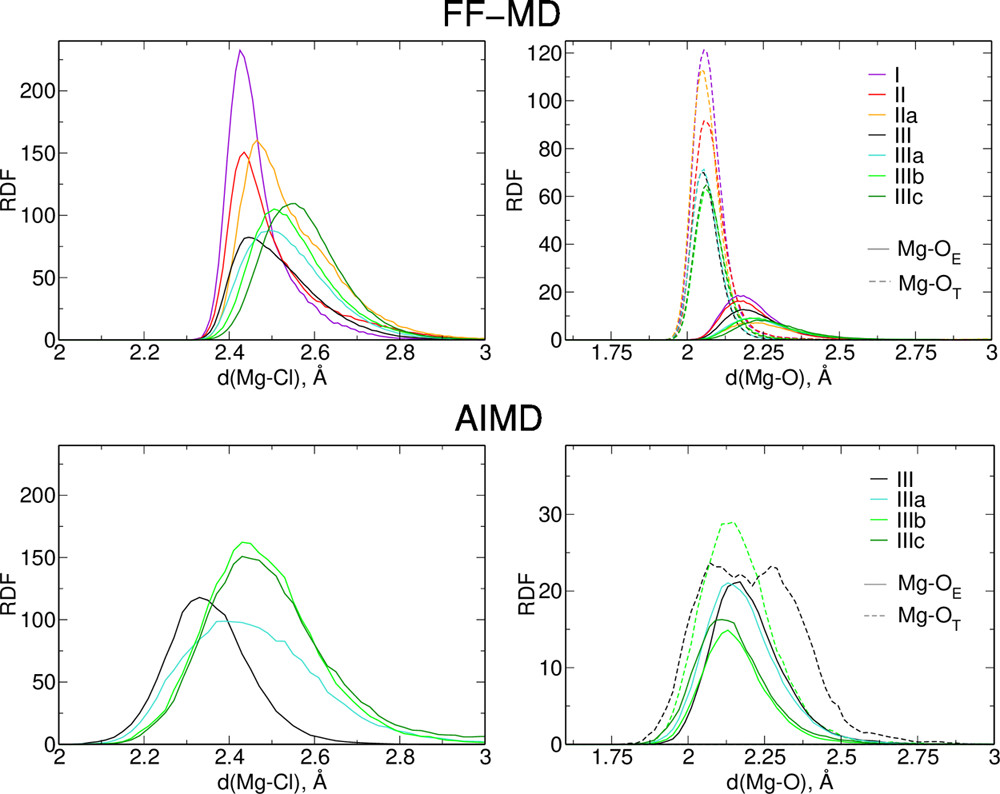
\includegraphics[width=0.6\textwidth]{img/3-structural-data-from-md-simulations/3-mg-cl-dme/rdf-mg-cl-o.png}
    \caption{Radial distribution functions for Mg-Cl and Mg-O distances (O$_{\text{E}}$ - oxygen from DME, O$_{\text{T}}$ - oxygen from TFSI$^{-}$)}
    \label{fig:mg-cl-dme-rdf-mg-cl-o}
\end{figure}

\begin{figure}[ht]
    \centering
    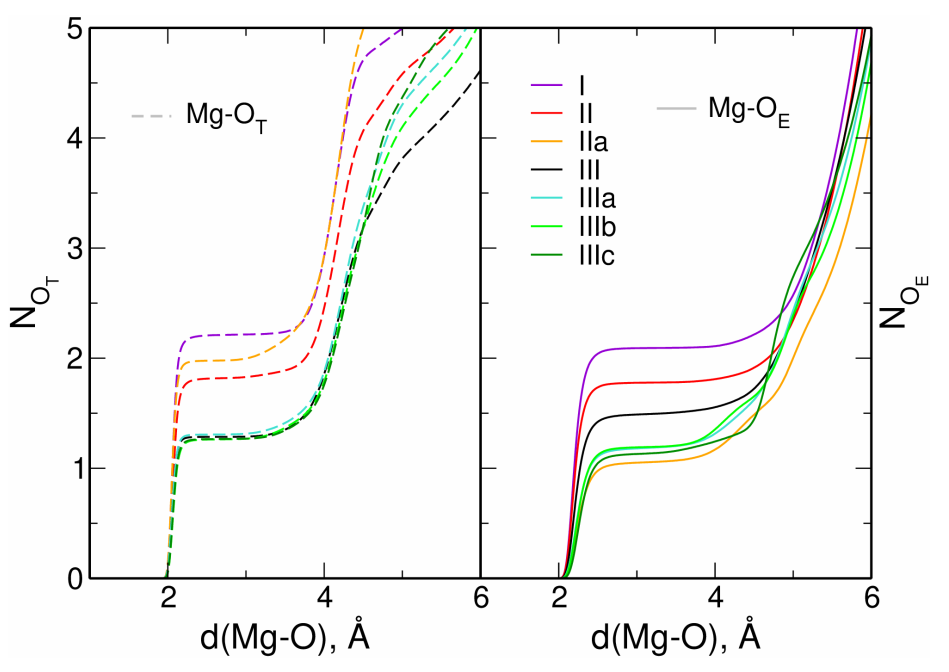
\includegraphics[width=0.6\textwidth]{img/3-structural-data-from-md-simulations/3-mg-cl-dme/rdf-int-mg-o.png}
    \caption{Integrated RDFs for Mg-O pairs from classical MD simulations, O$_{\text{E}}$ - oxygen atoms from DME, O$_{\text{T}}$ - oxygen atoms from TFSI$^{-}$)}
    \label{fig:mg-cl-dme-rdf-int-mg-o}
\end{figure}

The RDFs for the Mg-Cl and Mg-O distances obtained in MD simulations are plotted in Figure~\ref{fig:mg-cl-dme-rdf-mg-cl-o}. In the results of classical MD, the first maximum for Mg-Cl appears between 2.4 and 2.6~{\AA} and is larger for systems IIIa-c, which is consistent with the results of QC calculations where Mg-Cl distance was growing with increasing number of Mg$^{2+}$ ions in the complex. AIMD results show the same pattern, with the maxima shifted to distances shorter about 0.1~{\AA}. Classical MD trajectories were long enough to observe the coordination of the Mg$^{2+}$ ions by oxygen atoms both from the solvent and from the TFSI$^{-}$ anion, with the maxima positions again in the range that is consistent with the QC results. Integrated Mg-O RDFs, presented in Figure~\ref{fig:mg-cl-dme-rdf-int-mg-o}, show that oxygen atom coordination decreases from the most diluted system I~to systems IIIa-c where initially there were Mg-Cl complexes. This conclusion is confirmed by the integrated RDFs presented in Figure~\ref{fig:mg-cl-dme-rdf-int-mg-cl}, where an opposite trend is observed in the plot for Mg-Cl pairs.

\begin{figure}[ht]
    \centering
    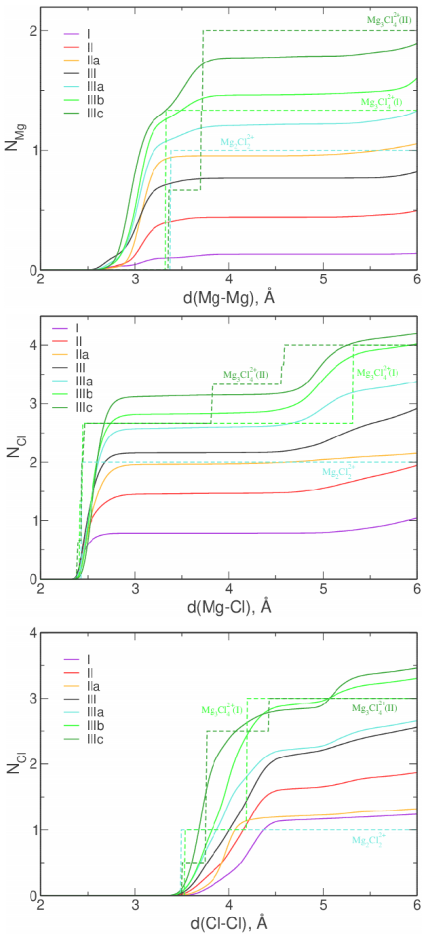
\includegraphics[width=0.45\textwidth]{img/3-structural-data-from-md-simulations/3-mg-cl-dme/rdf-int-mg-cl.png}
    \caption{Integrated RDFs for Mg-Mg and Mg-Cl pairs from classical MD simulations. Broken lines mark RDFs for "ideal" geometries of aggregates optimized in QC calculations}
    \label{fig:mg-cl-dme-rdf-int-mg-cl}
\end{figure}

\begin{figure}
    \centering
    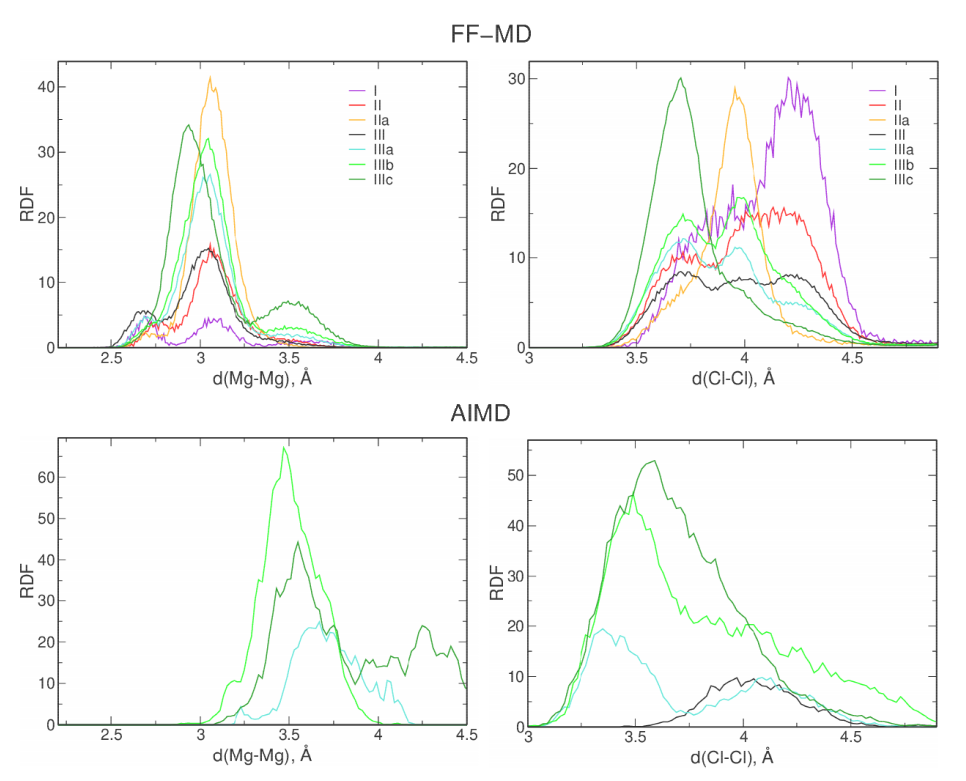
\includegraphics[width=0.75\textwidth]{img/3-structural-data-from-md-simulations/3-mg-cl-dme/rdf-mg-mg-cl-cl.png}
    \caption{Radial distribution functions for Mg-Mg and Cl-Cl pairs}
    \label{fig:mg-cl-dme-rdf-mg-mg-cl-cl}
\end{figure}

In Figure~\ref{fig:mg-cl-dme-rdf-mg-mg-cl-cl} RDFs for Mg-Mg and Cl-Cl pairs are presented. The main maximum in the Cl-Cl RDF is located at distances higher for systems I and II than for IIIa-c, which may be related to the QC results showing in Mg$_2$Cl$_2^{2+}$ the Cl-Cl distance longer than in the other complexes. Thus, it could be expected that in these systems the amount of this complex is significantly larger than that for IIIa-c. In AIMD, the positions of the maxima in Mg-Mg and Cl-Cl RDFs agree with the distances calculated by the QC methods. There is a~difference with respect to the results from classical MD. In classical MD the Mg-Mg maximum appears at shorter distances and Cl-Cl maximum at larger distances than in AIMD. As there are no significant differences in Mg-Cl RDFs, this may be related to different shapes of Mg$_2$Cl$_2^{2+}$ complex in both MD approaches, with the diagonal distance Mg-Mg longer and Cl-Cl shorter in AIMD.

\begin{figure}[ht]
    \centering
    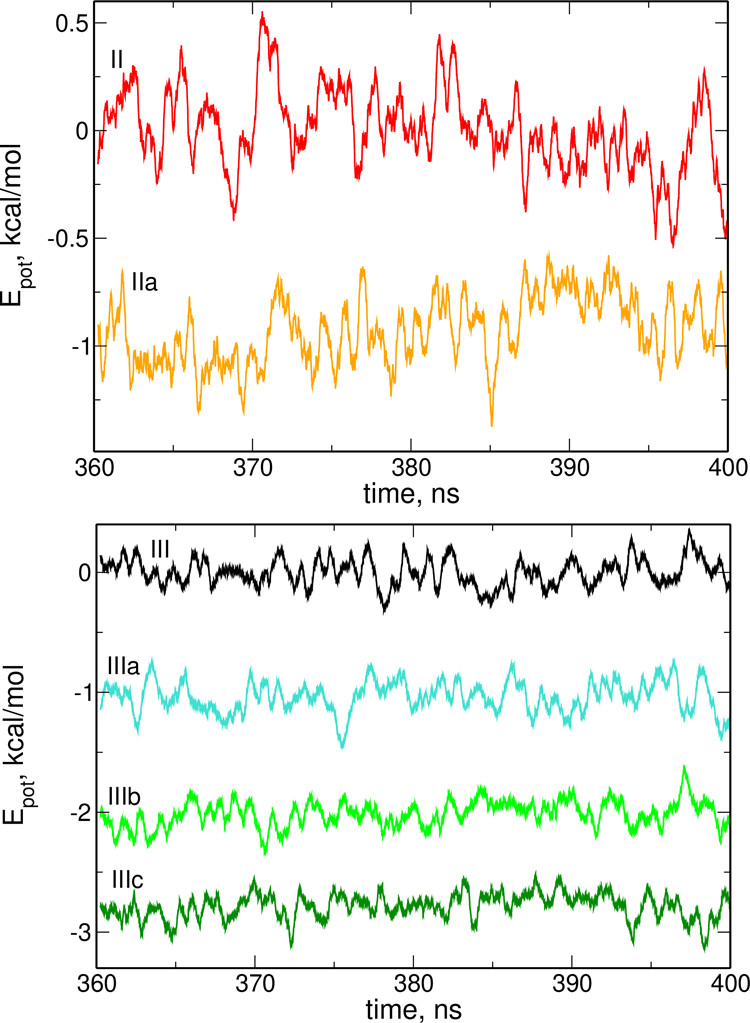
\includegraphics[width=0.5\textwidth]{img/3-structural-data-from-md-simulations/3-mg-cl-dme/energies.png}
    \caption{Relative potential energies $E_{\text{pot}}$ per Mg$^{2+}$ ion for II, IIa and III, IIIa-c systems for the last 40~ns of classical MD simulations with applied moving average over 0.5~ns.}
    \label{fig:mg-cl-dme-energies}
\end{figure}

Systems II and IIa contain the same number of ions and solvent molecules, the same applies for systems III and IIIa-c. To check which configuration of complexation is more stable, the relative potential energies for these systems are plotted in Figure~\ref{fig:mg-cl-dme-energies}. System IIa has energy lower than the system II, what suggests that in this case ion aggregation into Mg$_2$Cl$_2^{2+}$ is preferred. For the second series of systems, the energy decreases in order of III > IIIa > IIIb > IIIc, what suggests that complexation into Mg$_2$Cl$_2^{2+}$ and Mg$_3$Cl$_4^{2+}$ is favorable and that the II type of the Mg$_3$Cl$_4^{2+}$ complex is more stable than type~I.

\begin{figure}[ht]
    \centering
    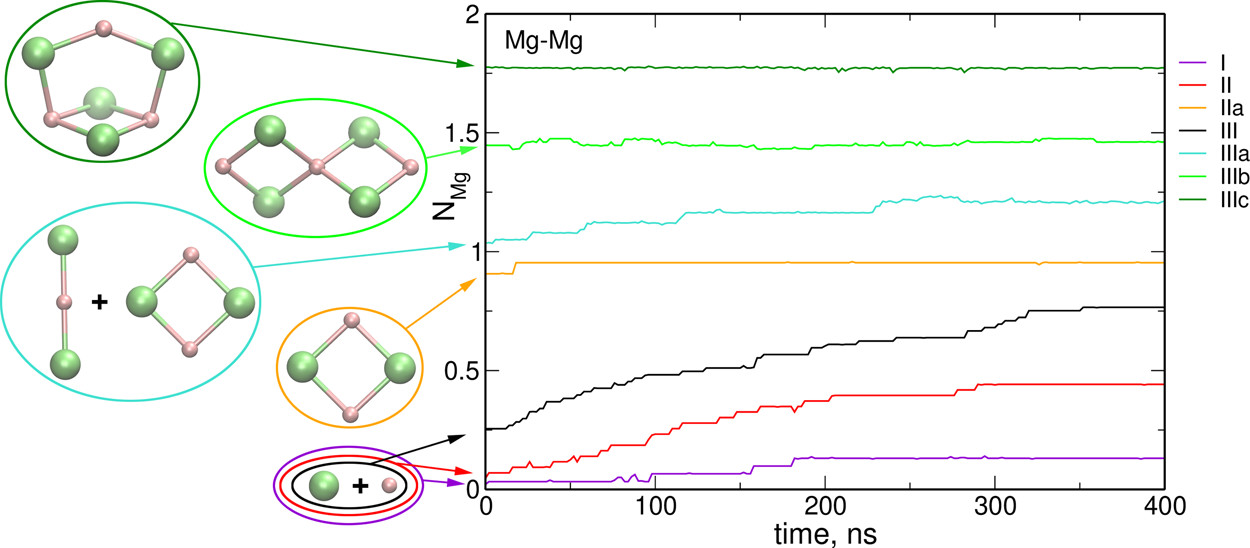
\includegraphics[width=0.75\textwidth]{img/3-structural-data-from-md-simulations/3-mg-cl-dme/average-mg.png}
    \caption{Average number of Mg$^{2+}$ ions at the distance of 4~{\AA} from the Mg$^{2+}$ ion. Initial arrangements of Mg$^{2+}$ and Cl$^{-}$ ions are shown on the left hand side of the plot}
    \label{fig:mg-cl-dme-average-mg}
\end{figure}

In Figure~\ref{fig:mg-cl-dme-average-mg} changes of average number of Mg$^{2+}$ ions at the distance of 4~{\AA} from the central Mg$^{2+}$ cation (N$_{\text{Mg}}$) are plotted for each system studied by classical MD. For systems which initially contained the preferred structure of the complex (i.e.~Mg$_2$Cl$_2^{2+}$ for the 1:1~ratio and Mg$_3$Cl$_4^{2+}$~(I) or~(II) for the 3:4 ratio), there are only small changes of this number with no decrease, what indicates that there is no dissociation. For other systems N$_{\text{Mg}}$ increases with time what shows that the ion aggregation process is occuring in the electrolyte. The speed of this growth decreases over time, because for larger aggregates, the mobility is decreased and it requires larger time for the next aggregation process to occur.

For each system at 3~points of the classical trajectory - initial, after 20~ns and after 400~ns, the abundance of different forms of Mg$_x$Cl$_y$ complexes was determined. Results for systems I, II and IIa are in Figure~\ref{fig:mg-cl-dme-speciation-1} and for the other in Figure~\ref{fig:mg-cl-dme-speciation-2}. For system~I, where Mg(TFSI)$_2$:MgCl$_2$ ratio equals 2:1, there are less Cl$^{-}$ anions than metal cations, so at any time there must be some "free" magnesium ions present. This effect is observed - after 400~ns still more than 50\% of cations are not coordinated to chlorine anions. Initially, some amount of MgCl$^{+}$ complex is formed and then aggregates into more complicated structures: MgCl$_2$ and Mg$_2$Cl$_y^{4-y}$ with y > 2.

For system II, which at the first step contained only "free" Mg$^{2+}$, initially MgCl$^{+}$ and MgCl$_2$ are produced, and after 400~ns these complexes and "free" Mg$^{2+}$ cations are still present in the solution but MgCl$^{+}$ amount is smaller. Instead, Mg$_2$Cl$_y^{4-y}$ aggregates are formed. System IIa contained Mg$_2$Cl$_2^{2+}$ aggregate at first step, and initially within 20~ns some of them dissociated and some associated into larger aggregates, there are no significant further changes.

In systems III and IIIa-c the Mg(TFSI)$_2$:MgCl$_2$ ratio is 1:2, so it is possible for all of the Mg$^{2+}$ cations to form Mg$_3$Cl$_4^{2+}$ complexes. In systems III and IIIa aggregation processes are observed. In the former, initially within 20~ns MgCl$^{+}$ and MgCl$_2$ are produced and then condense into more aggregated complexes with some amount of Mg$_3$Cl$_4^{2+}$. In system IIIa, the amount of initially present MgCl$_2$ and Mg$_2$Cl$_2^{2+}$ decreases and both types of Mg$_3$Cl$_4^{2+}$ are formed. For IIIb and IIIc only small number of initial complexes dissociate or associate into larger forms, and after that the amount of Mg$_3$Cl$_4^{2+}$ remains constant. However, in IIIb system, a~conversion of type I of Mg$_3$Cl$_4^{2+}$ into type II ist observed what remains in aggreement with QC results indicating bigger stability of type II.

\begin{figure}[H]
    \centering
    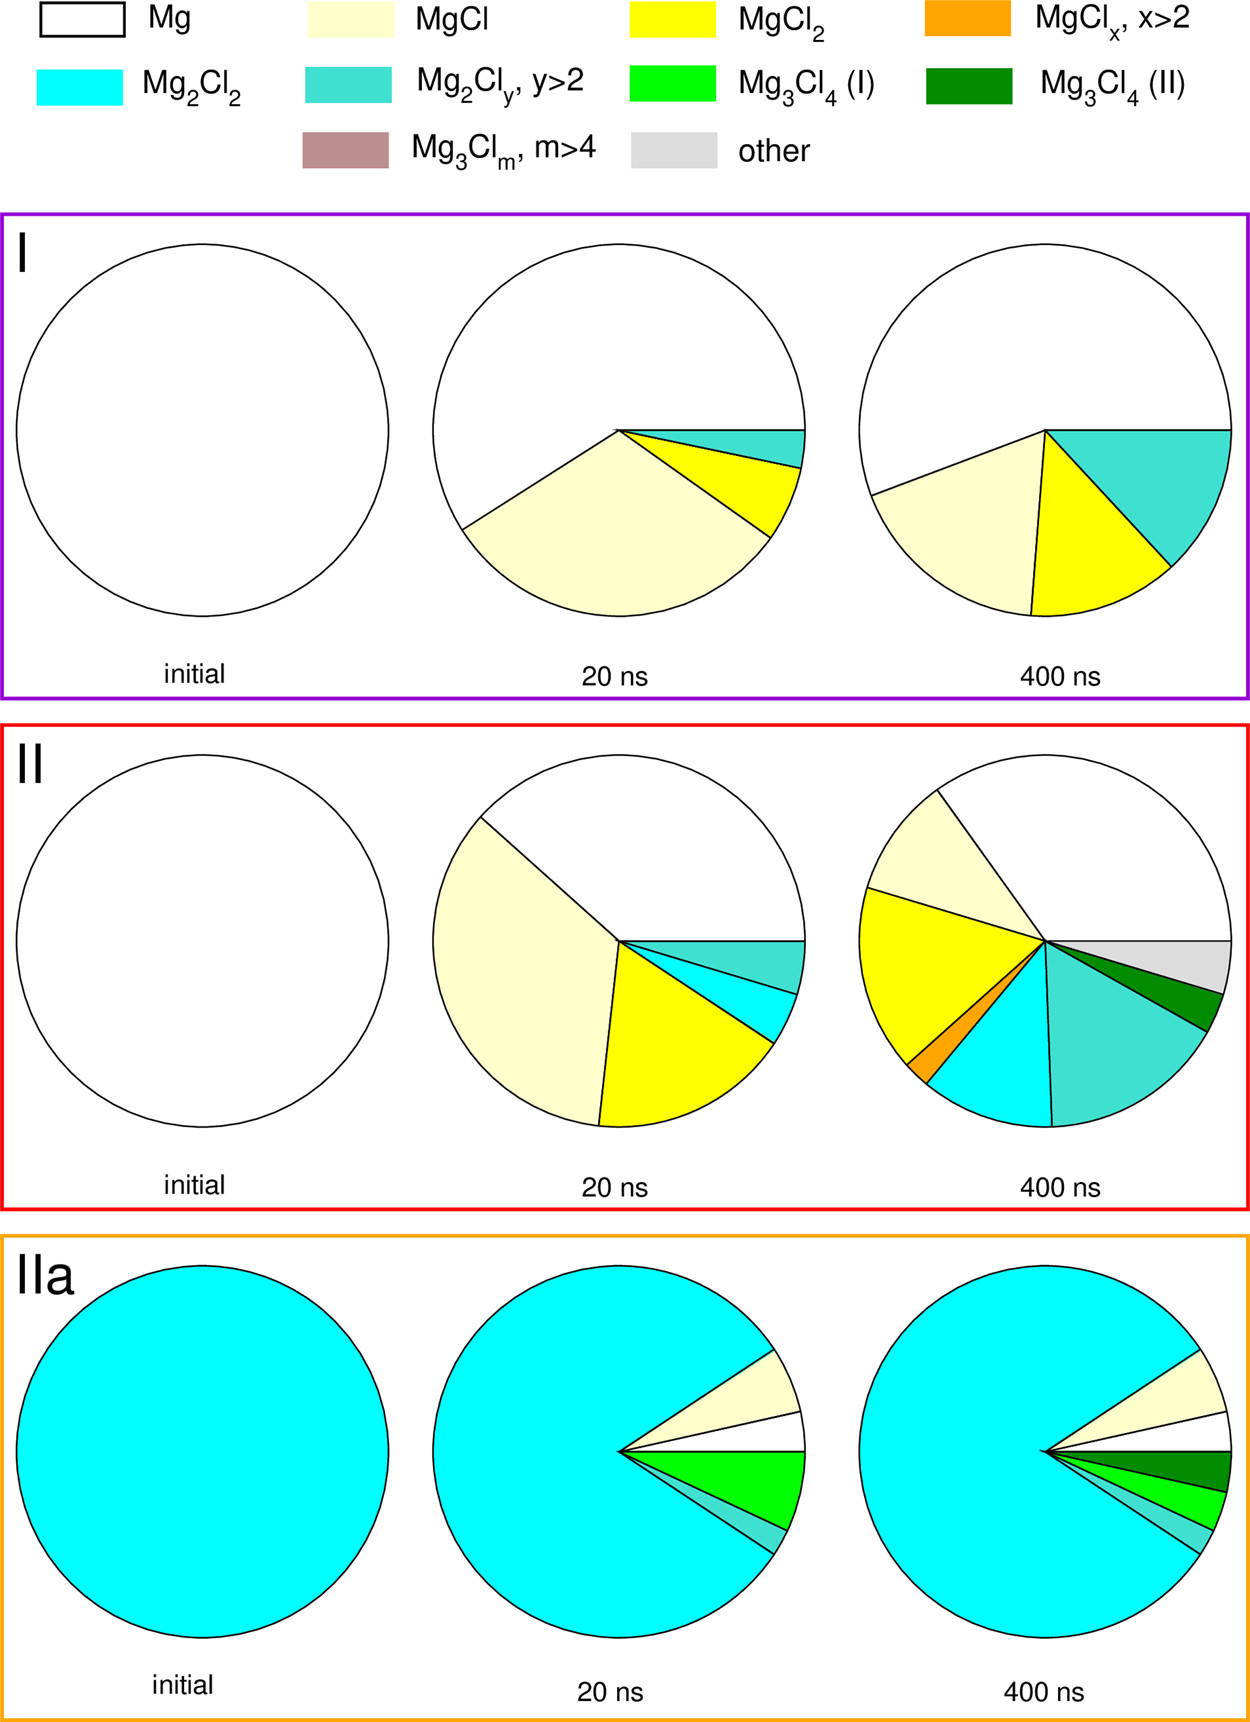
\includegraphics[width=0.5\textwidth]{img/3-structural-data-from-md-simulations/3-mg-cl-dme/speciation-1.png}
    \singlespacing
    \caption{Abundance of Mg$^{2+}$ ions in different complexes at different stages of classical MD simulations for systems I, II and IIa}
    \label{fig:mg-cl-dme-speciation-1}
\end{figure}

From these simulations it could by concluded that Mg$^{2+}$ ions tend to form stable Mg$_2$Cl$_2^{2+}$ or Mg$_3$Cl$_4^{2+}$ complexes, depending on the Mg(TFSI)$_2$:MgCl$_2$ ratio. The results support the conclusions of the experimental work~\cite{mg-dme-structures} about the possible processes of ion association occuring in the electrolyte.

\begin{figure}[ht]
    \centering
    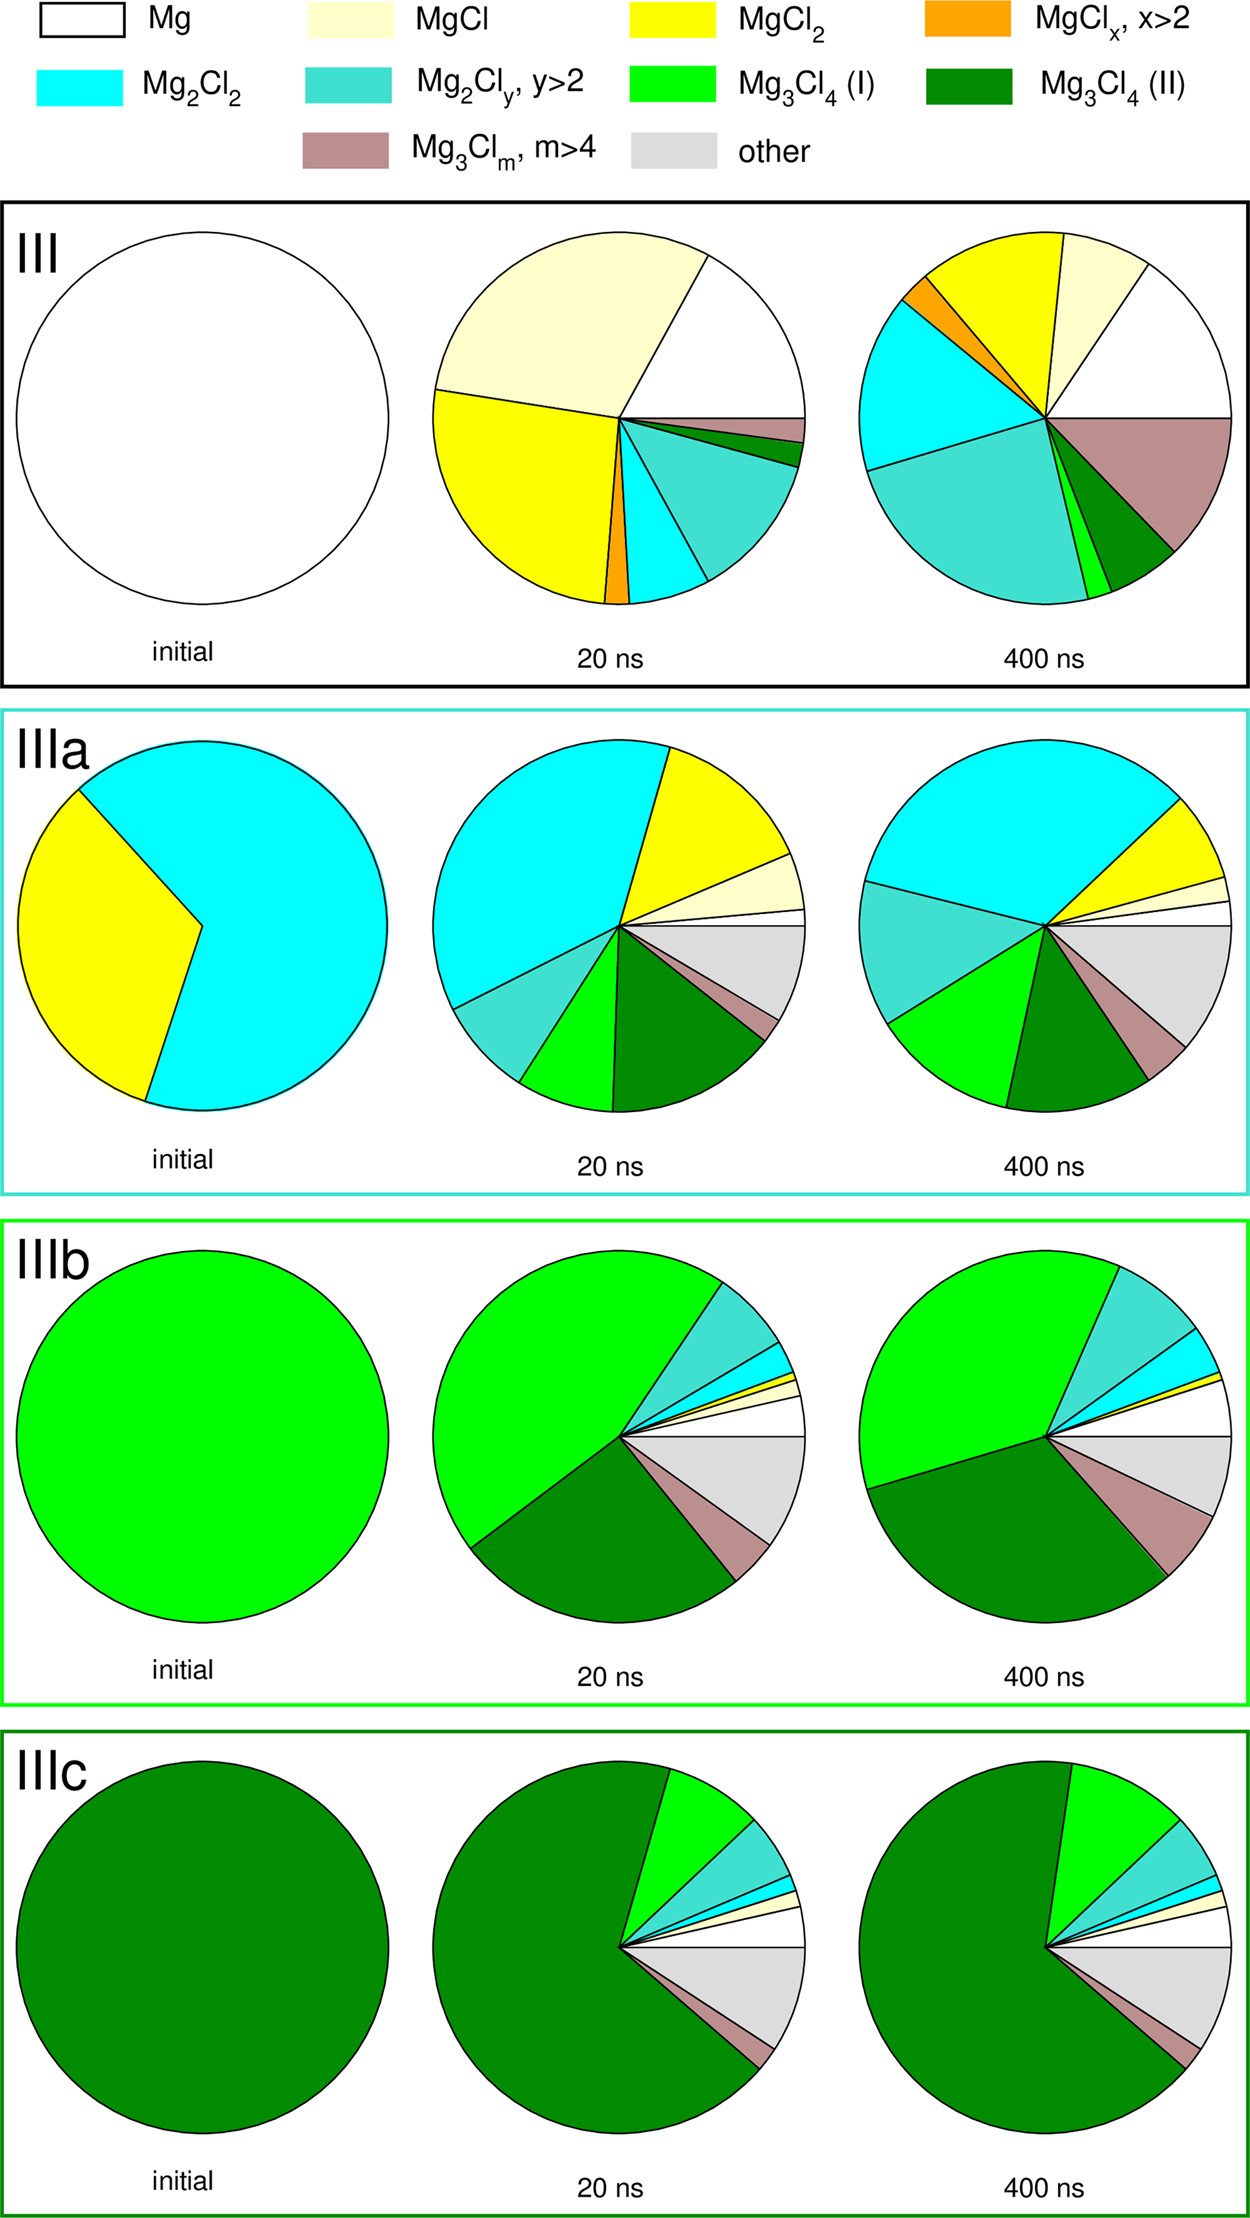
\includegraphics[width=0.5\textwidth]{img/3-structural-data-from-md-simulations/3-mg-cl-dme/speciation-2.png}
    \caption{Abundance of Mg$^{2+}$ ions in different complexes at different stages of classical MD simulations for systems III, IIIa, IIIb and IIIc}
    \label{fig:mg-cl-dme-speciation-2}
\end{figure}

\cleardoublepage